% This section provides a description of your product and defines it's
% primary features and functions. The purpose is to give the document
% reader/reviewer enough information about the product to allow them
% to easily follow the specification of requirements found in the
% remainder of the document. Your header for this section should
% introduce the section with a brief statement such as: "This section
% provides the reader with an overview of X. The primary operational
% aspects of the product, from the perspective of end users, maintainers
% and administrators, are defined here. The key features and functions
% found in the product, as well as critical user interactions and user
% interfaces are described in detail." Using words, and pictures or
% graphics where possible, specify the following:

This section provides the reader with an overview of MavDegreePlanner.
The primary operational aspects of the product, from the perspective
of end users and maintainers are defined here. The key features and
functions found in the product, as well as critical user interactions
and user interfaces are described in detail.

\subsection{Features \& Functions}
% What the product does and does not do. Specify in words what it looks
% like, referring to a conceptual diagram/graphic (Figure X).  Define
% the principle parts/components of the product. Specify the elements
% in the diagram/graphic that are part(s) of this product as well as
% any associated external elements (e.g., the Internet, an external
% web server, a GPS satellite, etc.)

The screen is divided into two parts, the website banner, the side
panel and the main screen. The side panel has a button to select a
major, a search bar, and the list of classes. The main screen has
the list of semesters and which classes the student has selected
for each. The website banner has the website logo, title, and
a button to go to the accounts page.

Accounts page where users can sign in, sign out, and reset password.
Users can create an account so that they can access their degree plan
from any device.

In the side panel, show a list of classes which are draggable,
and visually show which classes are required by the degree plan.
Choosing a major will show which classes are required for the student
to take. The classes can also be searched using the search bar above the list.

On the main screen, show a row of semesters which classes can be dragged to.
The list of semesters can be horizonally scrolled to show more semesters, and
have buttons to scroll for the user.
Classes are chosen by dragging and droping classes to the semester box.
There will be an error shown to the user if they choosen a class
without having the co-reg or pre-req class.

\subsection{External Inputs \& Outputs}
% Describe critical external data flows. What does your product
% require/expect to receive from end users or external systems (inputs),
% and what is expected to be created by your product for consumption by
% end users or external systems (outputs)? In other words, specify here
% all data/information to flow into and out of your systems. A table
% works best here, with rows for each critical data element, and columns
% for name, description and use.

\begin{table}[h]
    \resizebox{\textwidth}{!}{
        \begin{tabular}{|l|l|l|}
            \hline
            \textbf{Name} & \textbf{Description}                                           & \textbf{Use}                                 \\ \hline
            Courses       & (External Input) Maintainers will upload the list of classes   & List of classes that the user can signup for \\ \hline
            PDF           & (Output) PDF of the website to save the list of classes chosen & PDF of the classes chosen by the user        \\ \hline
        \end{tabular}}
    \caption{Overview of external inputs and outputs}
\end{table}

\subsection{Product Interfaces}
% Specify what all operational (visible) interfaces look like to your
% end-user, administrator, maintainer, etc. Show sample/mocked-up screen shots,
% graphics of buttons, panels, etc. Refer to the critical external inputs
% and outputs described in the paragraph above.

Administrators can use the Firebase backend. End-users can access to website
with an account, see the image below.

\begin{figure}[h!]
    \centering
    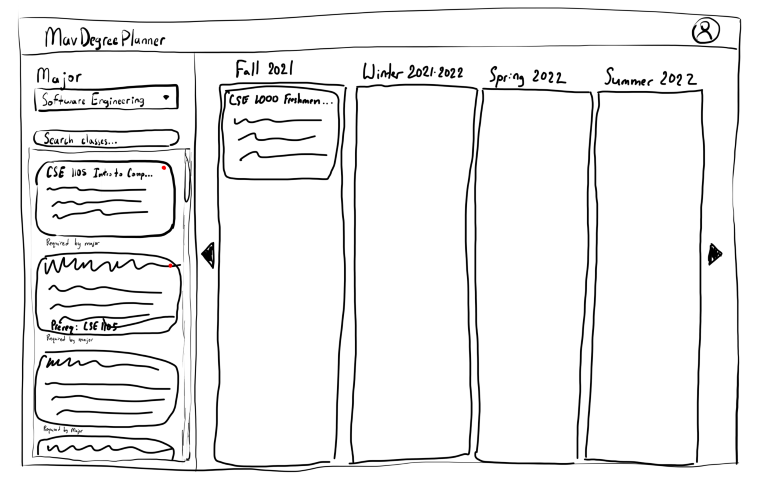
\includegraphics[width=0.60\textwidth]{images/MavDegreePlannerDiagram-Small}
    \caption{MavDegreePlanner Concept Sketch}
\end{figure}
